
\chapter{Fundamentação Teórica}

\section{Internet das Coisas}

O termo Internet das Coisas (em inglês, Internet of Things - IoT),
foi usado pela primeira vez em 1999 pelo pesquisador britânico Kevin
Ashton\cite{Ashton2009}. O autor descreve a Internet das Coisas como
um sistema através do qual os objetos do nosso cotidiano possam se
conectar à internet usando sensores. Ashton aplicou esse termo para
explicar o poder da conectividade das tags de rádio frequência identificada
(RFID), usadas pelas grandes empresas para contagem de estoques sem
a necessidade da interferência humana.

Em \cite{santos2014}, os pesquisadores definem IoT como “uma rede
de objetos interconectados, os quais poderiam possuir seus próprio
endereço de IP, estar incorporados a sistemas complexos e usar sensores
para monitorar o ambiente, respondendo a mudanças de contexto”. Tais
pesquisadores ainda avaliam a Internet das Coisas em quatro aspectos.
O primeiro é a possibilidade de seus sistemas conduzirem seus processos
de forma independente da Internet atual. O segundo é que a IoT é construída
em conjunto com novos serviços. O terceiro é que ela serve como ponte
de comunicação não somente entre pessoas e objetos, mas também entre
objetos e objetos (M2M ou Machine-to-Machine), e por último é que
as redes podem ser abertas (públicas) ou fechadas (privadas ou restritas
somente para alguns dispositivos).

A internet revolucionou a forma como as pessoas se comunicam em escala
global, o próximo passo é intercomunicar as ``coisas''. Os recentes
avanços na tecnologia de sistemas micro-eletro-mecânicos nas comunicações
sem fio e na eletrônica digital, possibilitaram a construção de microcontroladores
e sensores de tamanho e custo reduzidos. A proliferação destes dispositivos
em uma rede de comunicação cria a chamada Internet das Coisas (IoT).

Na última edição do IoT World Forum, realizada de entre 6 e 8 de dezembro
de 2015 em Dubai\cite{url:computerworld:2015,url:webintel:2015,url:cisco:iot:2015},
foram divulgados alguns dados que demostram o tamanho do crescimento
da IoT. Entre eles:
\begin{itemize}
\item 58\% das empresas do mercado dizem que IoT é estratégico para seu
futuro (se tiver, uma referência mais específica); 
\item Atualmente o crescimento de sistemas de IoT tem dobrado ano a ano; 
\end{itemize}
Crescimento da IoT entre 2013 e 2015:
\begin{itemize}
\item Sensores colocados no mercado: 10 bilhões em 2013 e 55 bilhões em
2015; 
\item Conexões de IoT: 11 bilhões em 2013 e 18 bilhões em 2015; 
\item Conexões M2M: 43 bilhões em 2013 e 73 bilhões em 2015; 
\item Empresas participantes em consórcios e associações da IoT: 44 em 2013
e 354 em 2015;
\end{itemize}
Investimentos:
\begin{itemize}
\item Desenvolvedores focados em IoT: 291 mil em 2013 e 813 mil em 2015; 
\item Startups em IoT: 127 em 2013 e 1.502 em 2015;
\item Investimentos de Capital de Risco: US\$1,1 bilhão em 2013 e US\$ 2
bilhões em 2015;
\end{itemize}
Oportunidades:
\begin{itemize}
\item Receita gerada por IoT: US\$ 548 bilhões em 2013 e US\$ 780 bilhões
em 2015; 
\item Receita de serviços de M2M: US\$ 79 bilhões em 2013 e US\$ 122 bilhões
em 2015;
\item “Coisas” não conectadas em 2013: 99,25\% e em 2015 98,85\%.
\end{itemize}
Previsão para o ano 2020:
\begin{itemize}
\item 50 bilhões de “coisas” conectadas; 
\item 6 dispositivos por pessoa;
\item US\$ 11 trilhões de dólares em novos negócios. 
\end{itemize}
Vários protocolos de aplicação divergentes têm sido propostos para
Internet das Coisas, incluindo CoAP, REST, XMPP, AMQP, MQTT, DDS e
outros. Cada protocolo incide sobre um aspecto específico das comunicações
da Internet das Coisas. A falta de um protocolo que possa lidar com
as exigências verticais de mercado de aplicações da Internet das Coisas,
incluindo máquina-a-máquina, máquina-servidor, e comunicações de servidor
para servidor resultou em uma fragmentação do mercado entre muitos
protocolos. Por sua vez, esta fragmentação é um obstáculo principal
no desenvolvimento de novos serviços que exigem a integração de múltiplos
serviços da Internet das Coisas para desbloquear novas capacidades
e proporcionar uma integração horizontal entre os serviços.

Diferentes organismos de normalização e grupos estão ativos na criação
de pilhas de protocolo mais interoperáveis e de normas abertas para
a Internet das Coisas. À medida que avançamos a partir do HTTP, TCP
e IP para uma pilha de protocolos específicos para Internet das Coisas,
eventualmente, nos deparamos com uma sopa de acrônimos de protocolos
sem fio, como ZigBee, RFID, Bluetooth, e BACnet às normas de protocolo
de última geração, tais como 802.15.4e, 6LoWPAN, RPL, e CoAP, que
tentam unificar as redes de sensores sem fio e a Internet\cite{electronicdesign:2016}. 

Por definição, a Internet das Coisas tem um enorme abrangência, que
pode ser difícil de atender através de um única solução. A IoT pode
ser dividida em cinco principais setores (Figura \ref{fig:iot-report}),
que seriam as principais verticais de adoção da IoT\cite{Goldman2014}:
dispositivos vestíveis (\emph{Wearables}), carros conectados, casas
conectadas, cidades conectadas e Industriais.

\begin{figure}
\begin{centering}
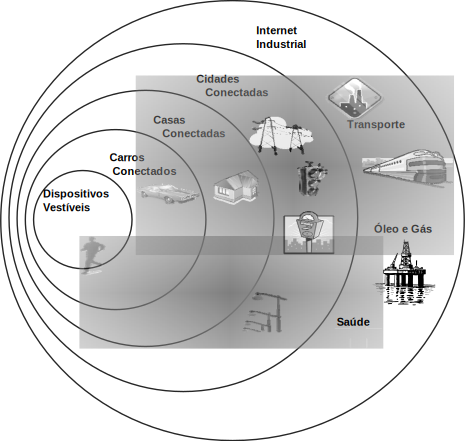
\includegraphics[width=0.7\linewidth]{Imagens/Cap_2/iot-report}
\par\end{centering}
\caption[Principais áreas de adoção]{ Principais áreas de adoção (traduzido e adaptado de \cite{Goldman2014})\label{fig:iot-report}}
\end{figure}

Na abertura do evento IoT Week 2013, Ashton afirmou que \textquotedbl{}A
IoT é aqui e agora; não é o futuro, mas o presente\textquotedbl{}\footnote{http://kevinjashton.com/2013/06/17/pre-recorded-opening-talk-for-internet-of-things-week-helsinki-
june-17-2013/}.


\section{Sistemas Embarcados}

Um sistema embarcado é uma combinação de hardware e software, projetados
para executar uma função específica \cite{Noergaar2005}. Como acontece
com qualquer sistema eletrônico, este sistema requer uma plataforma
de hardware construída com um microprocessador ou microcontrolador.
O hardware do sistema embarcado inclui elementos como interface do
usuário, interfaces de entrada/saída (I/O), display, memória, etc.
Geralmente, um sistema embarcado é composto por uma fonte de alimentação,
processador, memória, temporizadores, portas de comunicação serial
e circuitos específicos da aplicação do sistema.

Sistemas embarcados são mais limitados em hardware e software do que
um computador pessoal (PC). Em termos de limitações de hardware, isto
pode significar limitações no desempenho de processamento, o consumo
de energia, memória, e assim por diante\cite{Noergaar2005}.

\subsection{Tipos de Sistemas Embarcados}

Sistemas embarcados podem ser classificados em diferentes tipos: com
base no desempenho, requisitos funcionais e de desempenho do microcontrolador.

\begin{figure}[h]
\begin{centering}
\includegraphics[width=1\linewidth]{Imagens/Cap_2/embedded-systems-types}
\par\end{centering}
\caption{Tipos de Sistemas Embarcados \cite{url-efxkits} \label{fig:embedded-systems-types}}
\end{figure}

Sistemas embarcados são classificados em quatro categorias com base
em seu desempenho e requisitos funcionais:
\begin{itemize}
\item Sistemas embarcados autônomos;
\item Sistemas embarcados em tempo real; 
\item Sistemas embarcados em rede; 
\item Sistemas embarcados móveis.
\end{itemize}
Sistemas embarcados são classificados em três tipos, com base no desempenho
do microcontrolador, tal como:
\begin{itemize}
\item Sistemas embarcados de pequena escala; 
\item Sistemas embarcados de média escala; 
\item Sistemas embarcados sofisticados.
\end{itemize}
Neste trabalho, abordaremos com mais ênfase os sistemas embarcados
de pequena escala, compreendendo os microcontroladores, e os de média
escala, compreendendo os mini PCs.

\subsection{Microcontroladores}

Um microcontrolador é um sistema computacional completo, no qual estão
incluídos uma CPU (Central Processor Unit), memória de dados e programa,
um sistema de clock, portas de entrada/saída (I/O), além de outros
possíveis periféricos, tais como, módulos de temporização e conversores
A/D entre outros, integrados em um mesmo componente\cite{Chou1992}.

Os sistemas micro-controlados estão presentes nas mais diversas áreas,
dentre as quais estão a automação industrial, automação comercial,
automação predial, área automobilística, agrícola, produtos manufaturados,
eletrodomésticos, telecomunicações, etc. A Texas Instruments é creditada
com a criação do primeiro microcontrolador, a série TMS1000. Os microcontroladores
série TMS1000 tiveram bastante RAM, ROM e I/O e foram usados como
controladores de forno de micro-ondas, em temporizadores industriais,
e em calculadoras\cite{Gadre2000}.

Em geral, os microcontroladores são projetados para serem fáceis de
utilizar, do ponto de vista do projetista de circuitos. A Figura \ref{fig:microcontroller}
representa o diagrama de blocos do que um microcontrolador típico,
especialmente, os da série PIC. Um microcontrolador pode fazer interface
com motores, displays, leitura de sensores externos, realizar a comunicação
com um PC e mesmo se conectar a uma rede de controladores semelhantes,
e pode fazer tudo isso sem uma quantidade excessiva de componentes.
Isto leva a um pequeno e compacto sistema que é mais confiável e de
baixo custo.

\begin{figure}[h]
\begin{centering}
\includegraphics[width=0.8\linewidth]{Imagens/Cap_2/microcontrroler_pic}
\par\end{centering}
\caption{Diagrama de Blocos - PIC16F887 \cite{MilanVerle2008} \label{fig:microcontroller}}
\end{figure}

Em seguida, apresentamos os componentes do microcontrolador.
\begin{itemize}
\item \textbf{CPU:} A unidade central de processamento (CPU) é o coração
do controlador. Ela obtém as instruções armazenadas na memória de
programa, decodifica essas instruções, e executa. A CPU em si é composto
de registradores, a unidade lógica aritmética (ALU), decodificador
de instrução, e circuitos de controle.
\item \textbf{Memória de Programa}: A memória de programa armazena as instruções
que formam o programa. Para acomodar programas maiores, a memória
de programa pode ser particionada como memória de programa interno
e externo em alguns controladores. A memória de programa é geralmente
não volátil e pode ser EPROM, EEPROM, Flash, Mask ROM ou OTP (one-time
programmable).
\item \textbf{RAM}: A memória RAM é a memória de dados do controlador, ou
seja, ela é usada pelo controlador para armazenar dados. A CPU usa
memória RAM para armazenar variáveis, bem como a pilha. A pilha é
usada pelo processador para armazenar endereços de retorno a partir
de onde pode retomar a execução depois de ter completado uma sub-rotina
ou uma chamada de interrupção.
\item \textbf{Oscilador e Clock}: O controlador executa o programa a uma
determinada taxa. Esta velocidade é determinada pela frequência do
oscilador. O oscilador pode ser um oscilador RC-interno ou um oscilador
com um elemento de sincronismo externo, tal como um cristal de quartzo.
Assim que a energia é aplicada ao controlador, o oscilador começa
a funcionar.
\item \textbf{Porta Serial}: Ela é usada para se comunicar com dispositivos
externos através de uma comunicação serial, onde os dados são enviados
ou recebidos em 1 bit de cada vez. A porta serial pode operar em qualquer
velocidade de transferência, porém as mais usadas são 9800bps e 115200bps.
As portas seriais são de dois tipos: síncronas e assíncronas. A transferência
de dados síncrona precisa de um sinal de relógio (clock), para realizar
a ``sincronização'' do envio dos bits de dados, enquanto a transferência
de dados assíncrona não precisa do sinal do relógio, e a informação
de sincronização está incorporado nos dados, utilizando bits de controle
no início (START bit) e fim (STOP bit) do bloco de dados, que geralmente
é de 8-bits. O bit START é sempre baixo (0), enquanto o bit STOP é
sempre elevado (1).
\item \textbf{Porta I/O Digital}: O microcontrolador usa os componentes
de I/O (Entrada/Saída) digitais para a troca de dados digitais com
o mundo exterior. 
\item \textbf{Porta I/O Analógica}: A entrada analógica é realizada utilizando
um conversor analógico-digital (ADC). ADCs são usados para adquirir
dados analógicos de dispositivos, como sensores de temperatura e sensores
de pressão. A saída analógica é realizada utilizando um conversor
digital-para-analógico (DAC). A maioria dos controladores estão equipados
com moduladores de largura de pulso (PWM) que pode ser usado para
obter uma tensão analógica.
\item \textbf{Timer}: O \emph{timer} é usado pelo controlador para execução
de eventos baseados no tempo; por exemplo, realizar o controle de
velocidade de um motor, o brilho de um LED ou gerar um pulso PWM.
O \emph{timer} também pode ser usado para contar os eventos externos,
bem como internos, nesse caso, o temporizador é chamado um contador.
A quantidade de \emph{timers} disponíveis depende do microcontrolador
usado.
\item \textbf{Watchdog Timer}: O \emph{watchdog timer} (WDT) é um temporizador
especial, e geralmente é usado para prevenir falhas de software. Ele
funciona da seguinte forma: Uma vez armado, se o programa de usuário
não reiniciar o contador, notificando que tudo está certo, em um tempo
máximo predefinido, o contador estoura, ocorrendo o reset do microcontrolador.
A suposição é que, se o programa do usuário não repõe o WDT, ele falhou
de alguma maneira e, portanto, em vez de uma falha no sistema ou manter
um desempenho indesejado, é melhor reiniciar o sistema.
\end{itemize}

\subsection{Mini PCs}

Primeiramente, precisamos esclarecer que mini PCs não são os desktops
comuns, que já estão no mercado há alguns anos com placas-mãe pequenas
como micro ATX e flexATX. Estes, muito comuns em caixas de supermercado,
por exemplo, são apenas versões um pouco reduzidas dos computadores
comuns.

O tipo de máquina que estamos nos referindo são os credit-card sized
SBCs (single-board computers ou computadores de placa única do tamanho
de cartões de crédito). Além de serem super compactos, estes mini-pcs
foram desenhados especificamente para serem flexíveis e fáceis de
utilizar em projetos diversos por desenvolvedores, educadores e hobistas.
Suas dimensões não ultrapassam os 8 ou 9 centímetros de lado e, como
o nome já bem diz, possuem todos os seus componentes integrados em
uma única placa de circuito. São também muito eficientes no consumo
de energia, dispensando as complicadas e volumosas fontes dos PCs
comuns e utilizando portas USB ou carregadores padrão para sua alimentação.
Ainda assim, possuem opções de expansão e conectividade bem completas,
como entrada e saída de áudio, cartão SD, portas USB, saída HDMI e
rede ethernet.

Uma categoria especifica de mini PCs, voltada para desenvolvimento
de projetos embarcados, vem surgindo com o advento da Internet das
Coisas. Os avanços na tecnologia não permitiram apenas a miniaturização
dos computadores, permitiram também que seu custo fosse reduzido bastante.
Uma máquina como o Raspberry Pi custa apenas \$35 dólares. Outro modelo,
o BeagleBone Black custa a partir de \$45.


\subsection{Linguagens de Programação}

As linguagens de programação utilizadas em sistemas profundamente
embarcados incluem C, C++, e algumas vezes Java. É importante notar
que o Java é executado, na maioria das vezes, ``em cima'' de um
sistema operacional, o que limita (mas não impede) sua execução em
sistemas embarcados como microcontroladores. Java é atraente para
os dispositivos da Internet das Coisas, porque o número de desenvolvedores
Java em todo o mundo traz enorme potencial de crescimento para a indústria.
Oracle e ARM estimam que há cerca de 450 mil engenheiros de software
embarcado em todo o mundo, e cerca de nove milhões de desenvolvedores
Java\cite{java.com:2016}.

\section{Plataformas de Desenvolvimento\label{sec:Plataformas-de-Desenvolvimento}}

Nesta seção serão apresentadas algumas plataformas de desenvolvimento
de sistemas embarcados e prototipação, destacando as que tem ganhado
mais destaque na comunidade. A expansão da área de IoT tem estimulado
o desenvolvimento de novas ferramentas, plataformas de prototipação,
chips de comunicação, sensores e dispositivos diversos, abrindo o
leque de opções e reduzindo custos.

\subsection{Arduino}

Arduino\cite{url:arduino:intro} é uma plataforma de código aberto
usada para a construção de projetos eletrônicos. Arduino consiste
principalmente de uma placa de circuito físico programável (muitas
vezes referida como um microcontrolador) e um pedaço de software,
ou IDE (Integrated Development Environment), que é usada para escrever
e fazer upload de código (firmware) para a placa física\cite{url:arduino:intro}.

O Arduino tem o seu início no \emph{Interaction Design Institute},
na cidade de Ivrea, Itália, em 2005. O Professor Massimo Banzi estava
procurando uma maneira mais fácil e de baixo custo para ensinar os
estudantes de design a trabalhar com tecnologia. Ele discutiu o problema
com David Cuartielles, pesquisador visitante da Universidade de Malmö,
na Suécia, que estava à procura de uma solução semelhante, e o Arduino
nasceu\cite{arduino:evans:2013}. O conceito Arduino de hardware aberto
foi desenvolvido pela equipe visionária de Massimo Banzi, David Cuartielles,
Tom Igoe, Gianluca Martino, e David Mellis\cite{arduino:barrett:2012}.

Quando a maioria das pessoas pensam em Arduino, eles imaginam a pequena,
retangular (e provavelmente azul), placa de circuito impresso (PCB),
que é a parte fisicamente tangível do sistema Arduino. Tecnicamente
falando, o termo Arduino abrange o hardware, software, equipe de desenvolvimento,
a filosofia de design, e a comunidade de usuários. A Figura \ref{fig:arduino},
apresenta a placa Arduino, bem como, destaca seus principais componentes.

O Arduino foi originado do projeto Wiring\cite{Wiring:2016}, que
foi em si um ambiente de desenvolvimento de sistemas embarcados baseados
em AVR com uma IDE especializada escrita em Java. O Wiring, por sua
vez, foi originado do Processing\cite{Processing:2016}, outra coleção
de ferramentas de código aberto para escrever programas interativos
orientados a gráficos.

\begin{figure}[h]
\begin{centering}
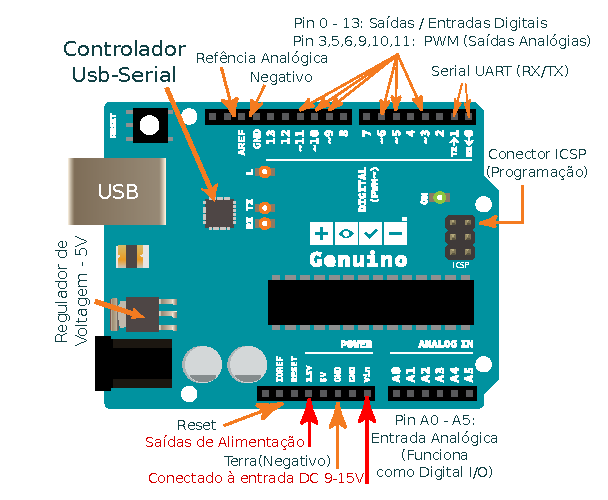
\includegraphics[width=0.8\linewidth]{Imagens/Cap_2/arduino}
\par\end{centering}
\caption[Placa Arduino ]{Placa Arduino (traduzido e adaptado de\cite{url:arduino:bord}) \label{fig:arduino}}
\end{figure}


\subsubsection{Características de Hardware}

O Arduino pode ser encontrado em várias versões, a maioria dos placas
são baseadas no microcontrolador Atmel AVR de 8 bits. A primeira placa
foi baseada na ATmega8 rodando a uma velocidade de clock de 16 MHz
com 8 KB de memória flash\cite{arduino:evans:2013}. Uma das placas
mais populares é o Arduino Uno\footnote{Arduino UNO (nos Estados Unidos) e Genuino UNO (fora dos Estados Unidos)},
que utilize o ATmega328p, com memória flash de 32KB e 2 KB de memória
RAM. Nos projetos mais exigentes, que requerem mais I/O e memória,
há o Arduino Mega 2560 com 256 KB de memória ou o Arduino Due\footnote{https://www.arduino.cc/en/Main/ArduinoBoardDue},
baseado no Atmel SAM3X8E ARM Cortex-M3, com 512KB de memória flash
e 96 KB de memória RAM.

As placas mais populares, em específico o Uno, têm 14 pinos digitais,
cada um dos quais podem ser definidos como entrada (input) ou saída
(output), e seis entradas analógicas. Além disso, seis dos pinos digitais
podem ser programados para proporcionar uma saída analógica PWM (Pulse
Width Modulation). Uma variedade de protocolos de comunicação estão
disponíveis, incluindo Serial, SPI (Serial Peripheral Interface),
e I2C (Inter-integrated Circuit Protocol). Na placa também é disponibilizada
uma entrada ICSP, que permite a programação do microcontrolador (que
é também realizada pela porta USB) e um botão de reset.

Placas especializadas chamadas \emph{Shields}, são usadas para expandir
as funcionalidade do Arduino. Estas podem ser empilhadas uma em cima
da outra para adicionar ainda mais funcionalidade, sendo esta, uma
das principais facilidades e fator de sucesso da plataforma Arduino.

\subsubsection{Características de Software}

Embora, muitas vezes o Arduino seja apresentado como uma linguagem,
na perspectiva de software, ele é na verdade um conjunto de bibliotecas
e APIs construídas em C/C++, que são baseadas nas APIs do projeto
Wiring.

A programação do Arduino é realizada por uma IDE (Integrated Development
Environment), escrita em Java e de código aberto\cite{arduino:source},
que fornece tudo que é necessário para a programação do Arduino, incluindo
uma série de programas de exemplo (sketches) que demonstram como conectá-lo
e se comunicar com alguns dispositivos comuns, como LEDs, LCDs, e
alguns sensores. 

A IDE do Arduino usa uma versão simplificada do C++\cite{arduino:ref},
tornando mais fácil aprender a programar e realizar interações com
o hardware. A estrutura básica de um programa para o Arduino é apresentado
na figura \ref{fig:arduino-1}. Programas escritos usando a IDE do
Arduino são chamados de sketches.

\begin{figure}[h]
\begin{centering}
\includegraphics[width=0.6\linewidth]{Imagens/Cap_2/arduinoide_sketch}
\par\end{centering}
\caption{IDE do Arduino \label{fig:arduino-1}}
\end{figure}


\subsection{Raspberry Pi\label{subsec:Raspberry-Pi}}

O Raspberry Pi\cite{url:raspberry} é um mini PC de baixo custo, do
tamanho de um cartão de crédito, que possui recursos consideráveis
de processamento e memória. Ele foi desenvolvido no Reino Unido, com
intuito de fomentar a educação para adultos e crianças e logo se destacou
na comunidade de desenvolvedores antes mesmo do seu lançamento oficial
em junho de 2012.

O equipamento usa como seu Sistema Operacional (S.O), a distribuição
Raspbian Wheezy, que é baseada no Linux Debian. Porém, existem inúmeros
Sistemas Operacionais compatíveis\cite{raspberry:compatible}, incluindo
o Windows 10 IoT Core\cite{raspberry:compatible1}. 


\subsubsection{Características de Hardware}

Existem diferentes modelos, que contemplam diferentes características
técnicas. O Raspberry Pi 2 Model B (Figura \ref{fig:raspberry})\footnote{ref:https://www.raspberrypi.org/products/model-b-plus/},
possui um processador com arquitetura ARM, 900MHz de velocidade (permitindo
overclock) e 1GB de memória RAM. O processador é o BCM 2835, o mesmo
usado no iPhone 3g e Kindle 2. 

\begin{figure}[h]
\begin{centering}
\includegraphics[width=0.8\linewidth]{Imagens/Cap_2/Raspberry_Pi_B}
\par\end{centering}
\caption{Raspberry Pi 2 - Model B \cite{img:raspberry} \label{fig:raspberry}}
\end{figure}


\paragraph*{Especificações:}
\begin{itemize}
\item SoC: Broadcom BCM2836 (CPU, GPU, DSP, SDRAM);
\item Processador: 900 MHz quad-core ARM Cortex A7 (ARMv7)
\item GPU: VideoCore IV @ 250 MHz / OpenGL ES 2.0 (24 GFLOFS);
\item Memória: 1GB MB (compartilhada com a GPU);
\item Saídas de Vídeo: 

\begin{itemize}
\item Vídeo Composto (PAL e NTSC) através de conector P2 com saída de áudio
integrada;
\item HDMI (ver 1.3 e 1.4);
\item Interface MIPI para ligar diretamente a painéis LCD.
\end{itemize}
\item Saídas de Áudio: Saída de áudio analógica através de conector P2 compartilhada
com o vídeo composto / HDMI;
\item Interfaces:

\begin{itemize}
\item 4 x portas USB 2.0;
\item 1 x MicroUSB (Alimentação);
\item 1 x Entrada MicroSD;
\item 1 x Ethernet (10/100Mbps);
\item 1 x GPIO (40 pinos) (General Purpose Input/Output).
\end{itemize}
\end{itemize}

\subsubsection{Características de Software}

Devido ao Raspberry Pi utilizar um S.O baseado em Linux e arquitetura
ARM, inúmeras linguagens de programação são suportadas\cite{raspberry:langs},
por exemplo, Java, JavaScript, PHP, Python, Ruby, etc. Bem como, é
possível executar servidores como Apache, Nginx e MySQL.

A distribuição oficial, Raspbian\cite{raspberry:os}, vem com suporte
nativo a Python e Java. A versão do Java instalada é a 'jdk-8-oracle-arm-vfp-hflt',
fornecida pela Oracle. É possível, contruir aplicações gráficas utilizando
\emph{JavaFX}\cite{raspberry:javafx}, tornando o Raspberry Pi, um
potencial equipamento para criação de inúmeras aplicações embarcadas.

Para controlar os pinos de GPIO em aplicações Java, existem várias
formas. Infelizmente a versão instalada não possui o suporte nativo
a este recurso (algo contraditório). Uma recente especificação, denomina
\emph{Device I/O}\cite{device-io:wiki}, foi projetada para acessar
os periféricos dos sistemas embarcados, permitindo acesso a recursos
como GPIO, I2C, SPI, UART, PWM, etc.

Para utilizar a API \emph{Device I/O}, é necessário instalar a versão
\emph{Java ME Embedded}\cite{device-io:wiki}, que conta com todos
componentes necessários. Porém, é possível utilizar API \emph{Device
I/O} com a versão do Java instalada por padrão no Raspberry Pi, necessitando,
neste caso, realizar a compilação da mesma.

Outra alternativa, é utilizar a biblioteca Pi4J\cite{raspberry:pi4j},
que permite realizar o acesso aos periféricos, utilizando uma API
Java totalmente orientada a objetos.


\subsection{BeagleBone}

A BeagleBone\cite{beagleboard} é outra plataforma na categoria de
mini PC, que se propõe a ser um computador de baixo custo, projetado
para fins educacionais. Ela foi projetado pela Texas Instruments,
e é totalmente open source, tanto em hardware quanto em software.

O equipamento usa como seu Sistema Operacional (S.O), a distribuição
Angstrom Linux, porém oferece suporte a outras versões do Linux, incluindo,
Debian, Ubuntu e Android.

\subsubsection{Características de Hardware}

Existem diferentes modelos, que contemplam diferentes características
técnicas. A BeagleBone Black (Figura \ref{fig:beaglebone}), possui
um processador AM3358BZCZ100, arquitetura ARM, 1Ghz de velocidade
e 512MB de memória RAM. Outros modelos podem chegar até 2GB de RAM.

Um dos diferencias em relação ao Raspberry Pi, é que ela possui uma
memória flash (eMMC) embutida de 4GB, onde é armazenado o Sistema
Operacional, o que permite um tempo carregamento do S.O menor (10s),
e maior confiabilidade do que o cartão MicroSD, utilizado no Raspberry
Pi.

Ao plugar a placa na porta USB do computador, ela é reconhecida como
um driver virtual de rede e pode ser acessada através do IP fixo\emph{
'http://192.168.7.2}'.

\begin{figure}[h]
\begin{centering}
\includegraphics[width=1\linewidth]{Imagens/Cap_2/beaglebone}
\par\end{centering}
\caption{BeagleBone Black \cite{img:BeagleBone} \label{fig:beaglebone}}
\end{figure}


\paragraph*{Especificações:}
\begin{itemize}
\item Processador: TI Sitara™ AM3358 ARM\textregistered{} Cortex™-A8
\item GPU: Suporte a aceleração gráfica 3D;
\item Memória: 512MB DDR3;
\item Armazenamento: 4GB 8-bit eMMC Onboard Flash;
\item Saídas de Vídeo: Micro HDMI;
\item Saídas de Áudio: Micro HDMI;
\item Interfaces:

\begin{itemize}
\item 1 x portas USB 2.0;
\item 1 x MicroUSB (Alimentação e Comunicação);
\item 1 x Entrada MicroSD;
\item 1 x Ethernet;
\item 2 x GPIO (46 pinos) (General Purpose Input/Output).
\end{itemize}
\end{itemize}

\subsubsection{Características de Software}

Devido ao S.O ser baseado em Linux, as principais linguagens de programação
são suportadas. A distribuição oficial, Angstrom, vem como uma IDE
Web (baseada na Cloud9 IDE\footnote{https://c9.io/} e Node.JS), que
permite executar programas em JavaScript utilizando Node.js e a biblioteca
BoneScript. A biblioteca BoneScript, permite o acesso aos periféricos
e pinos de GPIO da placa, possui uma sintaxe simples, com algumas
funções similares ao Arduino.

O desenvolvimento de aplicações usando Java é suportado, porém, é
necessário instalar o Java JDK 1.8 SE para plataforma ARM. Infelizmente,
não está disponível até o momento, a versão \emph{Java ME Embedded
}para a BeagleBone\emph{, }que oferece suporte a API \emph{Device
I/O.} A alterativa, neste caso, é compilar a biblioteca. Apesar do
site do projeto \emph{Device I/O,} não mencionar a compatibilidade
com a esta placa, nos testes efetuados, a compilação foi realizada
com sucesso e o acesso aos pinos GPIO pode ser realizado através do
Java\emph{.}

Outra alternativa, é utilizar a biblioteca ``libbulldog''\cite{beagleboard:libbulldog},
que permite realizar o acesso aos periféricos, utilizando uma API
Java totalmente orientada a objetos.


\subsection{ESP8266}

O ESP8266\cite{url:esp8266:espressif}\cite{esp8266:datasheet} é
um SoC (System on a Chip), altamente integrado, projetado para as
necessidades de um mundo cada vez mais conectado. Ele oferece uma
solução completa e independente de rede Wi-Fi, permitindo rodar aplicações
embarcadas ou fornecer as funções de rede Wi-Fi para outros microcontroladores,
através de uma comunicação serial UART. O ESP8266 tem poderosas capacidades
de processamento e armazenamento que permitem que ele seja usado com
sensores e outros dispositivos através de suas interfaces de GPIO
(General Purpose Input/Output). Seu alto grau de integração ``\emph{on-chip}'',
permite a simplificação dos projetos de circuitos. Toda a solução,
incluindo o módulo, está concebido para ocupar uma área mínima de
PCB (Printed Circuit Board). Um dos principais atrativos e fatores
de sucesso, é seu baixíssimo custo\footnote{https://www.sparkfun.com/products/13678}
e a facilidade com que o mesmo pode ser integrado a demais soluções,
tornando-se uma das plataformas mais populares de desenvolvimento
nos últimos anos.

\subsubsection{Características de Hardware}

O ESP8266 (Figura \ref{fig:esp8266}b) foi desenvolvido pela \emph{Espressif
Systems}, como uma interface Serial (UART) para Wi-Fi, usando o microcontrolador
\emph{Tensilica Xtensa LX3} de 32-bits, com clock de 80MHz, 32KB RAM
(instrução) e 96KB RAM (dados). O núcleo da CPU é baseado no Xtensa\cite{esp8266:cadence},
da Cadence.

Os módulos ESP8266 são fornecidos numa ampla variedade de modelos,
com diferenças perceptíveis principalmente no que tange à quantidade
de pinos I/O disponíveis para acesso externo, e no tamanho do módulo.
Até o presente momento, \textquotedbl{}oficialmente\textquotedbl{}
existem módulos numerados de ESP-01 até ESP-12\cite{esp8266:modules}.
A Figura \ref{fig:esp8266}a, apresenta o módulo ESP-01.

\begin{figure}[h]
\begin{centering}
\includegraphics[width=0.8\linewidth]{Imagens/Cap_2/esp8266}
\par\end{centering}
\caption[Placa ESP8266]{Módulo ESP-01 (a), Chip ESP8266 (b), adaptado de \cite{url:esp8266:espressif}.
\label{fig:esp8266}}
\end{figure}


\paragraph*{Algumas características do módulo Wireless ESP8266:}
\begin{itemize}
\item Conexão à redes padrão 802.11 B/G/N;
\item CPU que opera em 80MHz, com possibilidade de operar em 160MHz;
\item Pilha TCP/IP integrada;
\item Tensão de operação : 3.3 V;
\item Tem conectores GPIO, barramentos I2C, SPI, UART, entrada ADC, saída
PWM e sensor interno de temperatura;
\item Suporte a memória Flash Externa - 512 KB até 16MB;
\item Modos de operação : Cliente, Access Point, Cliente+Access Point;
\item Modos de segurança Wireless : OPEN/WEP/WPA\_PSK/WPA2\_PSK/WPA\_WPA2\_PSK;
\item Suporta comunicação TCP e UDP, com até 5 conexões simultâneas.
\end{itemize}

\subsubsection{Características de Software}

A Espressif disponibiliza um SDK completo para trabalhar com o ESP8266\cite{esp8266:sdk}.
No SDK são disponibilizados recursos para suporte à SSL, JSON, e a
biblioteca lwIP\footnote{http://savannah.nongnu.org/projects/lwip/},
tornando esta uma solução bastante completa para criação de projetos
para a Internet das Coisas. A empresa possui um repositório no GitHub\cite{esp8266:source},
onde disponibiliza exemplos de código para firmwares com RTOS e comandos
AT. 

Alguns dos módulos vêm pré-carregados com um firmware que os transformam
em \textquotedbl{}Pontes Serial-WiFi\textquotedbl{}, permitindo serem
configurados e controlados por outros microcontroladores (ex.: Arduino).
Para realizar essa ponte, a interface serial dos módulos obedece a
uma tabela de comandos, que seguem o padrão AT, que podem variar de
acordo com a versão do firmware. 

Um dos firmwares mais populares é o NodeMCU\cite{esp8266:nodemcu},
que permite programar o módulo usando a linguagem de programação LUA,
tornando prático, por exemplo, a criação de um servidor Web com acionamento
de GPIOs. Existe também a possibilidade de programar o ESP8266 usando
JavaScript, através do firmware Espruino\cite{esp8266:espruino},
porém ainda em versão Beta.

Outra opção disponível, é programar o ESP8266 utilizando as APIs do
Arduino. A IDE do Arduino oferece suporte para o ESP8266, permitido
utilizá-lo como se fosse um Arduino. O núcleo ESP8266 para Arduino\cite{esp8266:arduino}
vem com bibliotecas para se comunicar através do Wi-Fi, usando servidores
TCP e UDP, configurar servidores HTTP, mDNS, e fazer atualizações
remotas. Permite também utilizar o sistema de arquivos em memória
flash ou cartões SD e realizar comunicação usando protocolos UART,
SPI e I2C.

\section{Rede de Sensores Sem Fio (RSSF)}

A combinação de sensoriamento, processamento e comunicação de interface,
oferta milhares de aplicações potenciais que é o conceito principal
de rede de sensores sem fio\cite{hill2003}. Os nós de sensores sem
fio são unidades auto-suficientes que consistem em uma fonte de energia,
capacidades de comunicação, poder de computação e um atuador ou sensor.
Eles podem se comunicar entre si, coletar dados do ambiente ao redor
ou se conectar a uma estação base externa ou centro de controle remoto\cite{olafsen2007}. 

Os recentes avanços tecnológicos em circuitos integrados de baixa
potência e comunicações sem fio, permitiram a criação de dispositivos
cada vez menores, com baixo consumo de energia e com baixo custo,
tonando-se soluções eficientes para uso em aplicações de sensoriamento
remoto. A combinação desses fatores melhorou a viabilidade de utilizar
uma rede de sensores composta por um grande número de sensores inteligentes,
permitindo a coleta, tratamento, análise e disseminação de informações
valiosas\cite{akyildiz2002}.

RSSFs em geral caracterizam-se por possuir uma alta densidade de nós.
Vários sensores monitoram o mesmo fenômeno, gerando dados redundantes
e, muitas vezes, fornecendo à aplicação um nível de qualidade maior
do que o necessário. Como a maior fonte de consumo de energia nos
sensores é a transmissão de dados, grande parte dos esforços de pesquisa
em RSSFs visa propor soluções para obter e rotear os dados de forma
eficiente em energia, a fim de estender o tempo de vida global da
rede. Por um lado, há propostas cujo enfoque é minimizar o número
de transmissões e/ou o tamanho das mensagens, realizando o roteamento
eficiente em energia\cite{heinzelman2000,intanagonwiwat2000}. Por
outro lado, pesquisas recentes\cite{perillo2003:1,perillo2003:2},
mostram que, em vez de fornecer uma redundância de dados desnecessária
para a aplicação, a alta densidade de nós pode ser aproveitada para
obter significativa economia de energia. Vários métodos podem ser
empregados a fim de se obter essa economia. 

A seguir estão algumas propriedades de redes de sensores sem fio:
\begin{itemize}
\item \textbf{Auto-organização:} Os nós de sensores podem criar automaticamente
a rede e a posição dos nós não precisam ser pré-determinada. Uma rede
de sensores auto-organizáveis não tem nenhuma necessidade de se ligar
a uma rede estabelecida.
\item \textbf{Comunicação de curto alcance e encaminhamento multi-salto:}
Comunicação multi-salto em redes de sensores sem fio é esperada para
consumir menos energia do que a comunicação tradicional de salto único.
Como sabemos, a potência de transmissão requerida aumenta com a distância
entre o transmissor e o receptor. Consequentemente, muitos pequenos
saltos requerem menos energia do que um longo salto.
\item \textbf{Cooperação entre nós:} Por causa dos recursos limitados dos
nós, papéis diferentes são atribuídos para nós na rede para alcançar
uma rede de baixa potência.
\item \textbf{Topologia Dinâmica:} Na rede de sensores sem fio, nós podem
falhar e ficar \emph{off-line}\footnote{fora de operação} ou novos
nós podem ser adicionados na rede. Assim, a topologia da rede opera
de forma dinâmica.
\item \textbf{Recursos energéticos limitados, poder computacional e memória:}
Uma vez que uma rede de sensores sem fio é composta por pequenos dispositivos,
a rede sofre com limitações de recursos, por exemplo energia, poder
computacional e memória.
\end{itemize}
É geralmente reconhecido que os sensores e redes de sensores serão
uma parte significativa da IoT \cite{Luckenbach2005}. Os sensores
podem monitorar o mundo físico por detectar e medir diferentes tipos
de informações ambientais. Ao alimentar aplicações adequadas com esse
tipo de informação através de vários tipos de objetos do mundo físico,
a Internet passaria de \textquotedbl{}computadores interligados\textquotedbl{}
para \textquotedbl{}as coisas interligadas.\textquotedbl{} Redes inteligentes
sensíveis ao contexto estão se aproximando rapidamente da posição
de sistemas de rede integrados, onde o desenvolvimento de minúsculos
sensores e atuadores pode perfeitamente realizar tais redes em grandes
ambientes de fábrica, redes para automóveis, residências, escritórios
inteligentes e serviços de apoio social, incluindo os alertas sísmicos,
monitoramento de pacientes e sensíveis ao contexto em situações de
emergência \cite{Luckenbach2005}.

\section{RFID}

O RFID - \emph{Radio Frequency Identification}, ou, em tradução livre,
Identificação por Radiofrequência, não é uma tecnologia nova, ela
teve seu início com o físico escocês Sir Robert Alexander Watson-Watt
em meados de 1937\cite{nemoto2012}. Esta tecnologia foi primeiramente
usada em sistemas de radares na Segunda Guerra Mundial para avisar
com antecedência a presença dos aviões aliados ou inimigos e que permaneceu
restrito somente para uso militar até os anos 70. C.M Roberts, em
\cite{Roberts2006}, descreve essa tecnologia como um ``sistema de
transação e identificação de dados por proximidade eletromagnética''.
O autor também afirma que o RFID é um melhoria sobre os códigos de
barras em termos de comunicação por proximidade não ótica.

Um sistema RFID consiste em leitores (também chamados de interrogadores)
e etiquetas (ou \emph{transponders}). Um sistema típico, tem alguns
leitores, estacionários ou móveis e muitas etiquetas que estão ligadas
a objetos, tais como livros, caixas de papelão, garrafas, etc\cite{Chawla2007}.
Um leitor se comunica com as etiquetas sem utilizar fios, dentro do
seu campo de atuação, e coleta informações sobre os objetos aos quais
as etiquetas estão associadas. Dependendo do seu princípio de funcionamento,
as etiquetas são classificados em três categorias: passivas, semi-passiva
e ativa.

A etiqueta passiva é a menos complexa e, portanto, a mais barata.
Não tem nenhuma fonte de alimentação interna, e usa o campo eletromagnético
transmitido por um leitor para alimentar seu circuito interno. Ela
não se baseia em um transmissor, mas em \textquotedbl{}retrodifusão\textquotedbl{}
para transmitir dados de volta para o leitor. A etiqueta semi-passiva
tem fonte de energia própria, mas nenhum transmissor, usando o mecanismo
de \textquotedbl{}retrodifusão. Uma etiqueta ativa, tem tanto fonte
de alimentação interna quando transmissor\cite{Chawla2007}.

A figura \ref{fig:rfid} ilustra o funcionamento do sistema RFID passivo
que consiste de uma etiqueta RFID e uma estação de base chamado \textquotedbl{}leitor
RFID\textquotedbl{}. Uma etiqueta passiva consiste em uma antena e
um circuito integrado de aplicação específica (ASIC), ambos com impedâncias
complexas. O chip obtém energia a partir do sinal de RF transmitido
pelo leitor RFID. A etiqueta envia dados de volta ao mudar a sua impedância
de entrada entre dois estados e modulando assim o sinal por \textquotedbl{}retrodifusão\textquotedbl{}. 

\begin{figure}[h]
\begin{centering}
\includegraphics[width=0.5\linewidth]{Imagens/Cap_2/rfid}
\par\end{centering}
\caption{Visão geral do RFID passivo \cite{Chawla2007}\label{fig:rfid}}
\end{figure}

Atualmente, o RFID tem uma gama enorme de aplicabilidade, que vão
desde os conhecidos cartões de acesso residenciais por proximidade
até ao rastreamento em cadeias de produção, controle estacionamento
de veículos, gerenciamento de estoque, rastreamento de livros, prevenção
de roubos, etc\cite{Roberts2006}.

Esta tecnologia tem se difundido rapidamente pelo mundo, por sua facilidade
de uso e também pelo fato de dispensar a intervenção humana\cite{zhu2012review}.
no mundo dos negócios o RFID tem recebido grande expectativas com
previsão de crescimento de US\$ 4,96 bilhões em 2007 e US\$ 26,88
bilhões em 2017\cite{RFIDForecasts2007}.

O RFID possibilitou a inserção de inteligência nos objetos, trazendo
aos mesmos a capacidade de comunicarem-se de forma automática\cite{Khoo2010}.
Em \cite{Khoo2010}, o autor afirma que o RFID representa uma tecnologia
que possibilitou a convergência entre computação, comunicação e interação
através de redes sem fio, sensores e a grande rede de computadores.
Em complemento o autor afirma que esta tecnologia tem o potencial
que permite a máquina identificar objetos, compreender seus estados
e tomar medidas, se necessário. Ou seja, possibilitou aos objetos
do nosso cotidiano pensar e interagir. Todo esse desenvolvimento contribuiu
com a criação da Internet das Coisas (IoT), que permite a interação
inteligente entre objetos ao redor do mundo. As soluções categorizadas
de acordo com o domínio de redes de sensores e a tecnologia RFID têm
abordado de forma eficiente problemas relacionados a interoperabilidade,
escalabilidade, infraestrutura distribuída, interação espontânea\cite{Luckenbach2005}. 

\section{Tecnologias de Comunicação}

A Internet das Coisas necessita de tecnologias de comunicação na camada
física e do middleware para fornecer o controle dos dispositivos para
a camada das aplicações. Tipicamente, os meios físicos de comunicação
entre os dispositivos são baseados em três grupos diferentes: cabeamento
estruturado, a fiação existente, e sem fio\cite{ngo2007}.

Na maioria dos casos, os dispositivos usam a comunicação sem fio porque
os padrões de tecnologia sem fio estão em toda parte. A ampla disseminação
de redes sem fio em nossa vida diária está habilitado para os padrões
de comunicação, como Bluetooth, Zigbee, RFID, Wi-Fi e redes móveis
(3G/4G). Prevê-se uma combinação destas normas e tecnologias, afim
de construir ambientes inteligentes. Efetivamente, todas as tecnologias
sem fio que podem apoiar de alguma forma a transferência de dados
remotos, detecção e controle, são candidatas para inclusão no ambiente
de IoT.

\subsection{Tecnologias não IP}

\subsubsection{ZigBee}

ZigBee é uma tecnologia de rede sem fio desenvolvida pela ZigBee Alliance
para aplicações de baixa taxa de transmissão de dados e de curto alcance\cite{alliance2007}.
É uma especificação para um conjunto de rede, segurança, e camadas
de software de aplicações baseado no padrão IEEE 802.15.4 para redes
de área pessoal (PAN)\cite{hwang2012}.

A pilha do protocolo ZigBee é composta de quatro camadas principais:
a camada física (PHY), a camada de controle de acesso ao meio (MAC),
a camada de rede (NWK), e a camada de aplicação (APL). PHY e MAC de
ZigBee são definidos pela norma IEEE 802.15.4, enquanto o resto da
pilha é definido pela especificação ZigBee.

ZigBee é especialmente adequado para aplicações em sensores, incluindo
automação predial, interruptores de luz sem fio, medidores elétricos
e sistemas de gestão de tráfego. Em geral, é indicado para aplicações
em que altas taxas de transferências de dados não são requeridas.
A versão inicial do IEEE 802.15.4, em que ZigBee é baseado, atua nas
frequências de 868MHz, 915 MHz e 2,4 GHz, que estão disponíveis na
Europa, América do Norte e em todo o mundo, respectivamente. As taxas
de dados são 20 kb/s, 40kb/s, e 250kb/s, respectivamente\cite{gomez2010wireless}.

Os perfis de aplicações ZigBee mais importantes são o \emph{ZigBee
Home Automation Public Application Profile}\cite{alliance2007} e
do \emph{ZigBee Smart Energy} Profile\cite{alliance11smart}. As principais
áreas de aplicação para o perfil \emph{Home Automation} são de iluminação,
controle de temperatura, e segurança. O perfil \emph{Smart Energy}
lida com aplicações de gerenciamento de demanda de energia e de gestão
de carga para as redes de energia.

\subsubsection{Bluetooth}

Bluetooth, definido pela norma IEEE 802.15.1\cite{Bluetooth2004}
foi inventado pelo provedor de telecomunicações Ericsson em 1994,
e foi originalmente concebido como uma alternativa sem fios para a
comunicação por fios RS-232. É um protocolo projetado principalmente
para baixo consumo de energia com um curto alcance. Opera mundialmente
através de uma banda de frequência não licenciada (ISM) em 2.4 GHz
(2400-2483,5 MHz), com taxas de transmissão de 1 Mbit/s \cite{Haartsen:1998}.
A figura \ref{fig:bluetooth_stack} apresenta a pilha do protocolo
Bluetooth.

O sistema Bluetooth provê conexões ponto-a-ponto (apenas dois dispositivos
Bluetooth envolvidos), ou conexões ponto-multiponto. Nas conexões
ponto-multiponto, o canal é compartilhado entre alguns dispositivos
Bluetooth, formando uma piconet. Em uma piconet, um dos dispositivos
Bluetooth funciona como master (mestre), enquanto os demais funcionam
como slaves (escravos). O master controla o acesso dos dispositivos
slaves, determina o clock responsável pela sincronização, dentre outras
funções.

A figura \ref{fig:bluetooth_net} apresenta alguns exemplos de topologias
possíveis. Em \ref{fig:bluetooth_stack}a, tem-se uma piconet com
um único escravo. Em \ref{fig:bluetooth_stack}b, tem-se uma piconet
com múltiplos escravos. Em \ref{fig:bluetooth_stack}c, tem-se uma
possível configuração de uma scatternet\cite{BluetoothSpecv1}.

Bluetooth suporta ligações síncronas e assíncronas. O link síncrono
orientado a conexão (SCO) é usado principalmente para voz e eles são
transmitidos através de intervalos reservados. O link para conexão
assíncrona (ACL) é usado principalmente para transmissão de dados.
Ligação ACL pode utilizar as faixas restantes no canal. Ao contrário
de SCO, para garantir a integridade de dados, no ACL pacotes são retransmitidos.

Existem três diferentes classes de dispositivos Bluetooth. Cada classe
tem uma potência de transmissão diferente (daí um alcance de transmissão
diferente)\cite{BluetoothCore}:
\begin{itemize}
\item Classe 1: O alcance de comunicação é de 100 metros e a potência de
transmissão é de 100 mW (20 dBm)
\item Classe 2: O alcance de comunicação é de 50 metros e a potência de
transmissão é de 2,5 mW (4 dBm)
\item Classe 3: O alcance de comunicação é de 10 metros e a potência de
transmissão é de 1 mW (0 dBm)
\end{itemize}
\begin{figure}
\begin{centering}
\includegraphics[width=0.4\linewidth]{Imagens/Cap_2/bluetooth_stack}
\par\end{centering}
\caption{Pilha do protocolo Bluetooth \cite{BluetoothCore} \label{fig:bluetooth_stack}}
\end{figure}

\begin{figure}
\begin{centering}
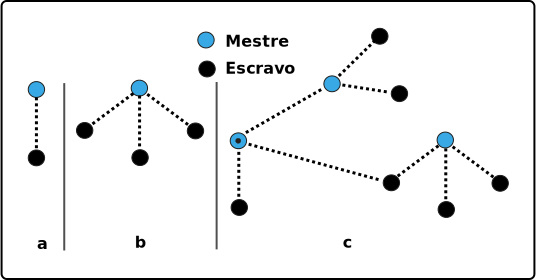
\includegraphics[width=0.6\linewidth]{Imagens/Cap_2/bluetooth_net}
\par\end{centering}
\caption[Topologias de redes Bluetooth]{Topologias de redes Bluetooth (traduzido de \cite{BluetoothSpecv1})
\label{fig:bluetooth_net}}
\end{figure}


\subsubsection{Bluetooth LE (Low Energy)}

Bluetooth \emph{Low Energy}, definido em \emph{Bluetooth Core Spec
4.0}\cite{bluetooth2010} e suas derivações 4.1 e 4.2, é um protocolo
sem fio operando na banda não licenciada de 2,4 GHz. Enquanto ela
opera na mesma faixa de frequência que outras tecnologias Bluetooth,
a sua operação nas camadas físicas (PHY) é incompatível, necessitando
de dispositivos com chipsets operem nos dois modos (Dual-mode)\cite{bluetooth2010}.
A camada PHY BT.LE usa \emph{Gaussian Frequency Shift Keying} (FSK)
com um deslocamento de 250 kHz. Ele transmite em um dos 40 canais
em 1 Mbit/s.

Segundo a Bluetooth SIG (Special Interest Group), o Bluetooth LE,
destaca-se como uma importante tecnologia para a Internet das Coisas:
\begin{quote}
Bluetooth 4.2 is an important update to the Bluetooth Core Specification
delivering exciting new features and benefits for Bluetooth Smart.
This will create significant advantages for developers and manufacturers,
while providing a better user experience for their customers. Bluetooth
4.2 makes Bluetooth Smart even smarter, faster and the ideal wireless
technology for the Internet of Things (IoT).\cite{bluetooth2010:site}
\end{quote}
Resumidamente as diferenças de aplicação entre as versões são destacadas
a seguir:
\begin{itemize}
\item Bluetooth BR/EDR (2.0/2.1): Estabelece uma distância relativamente
curta, conexão sem fio contínua, o que o torna ideal para os casos
de uso, tais como streaming de áudio. 
\item Bluetooth LE (4.0): Rajadas de conexão de rádio de longo alcance,
tornando-o ideal para a Internet das Coisas (IoT), aplicações que
não necessitam de conexão contínua, mas dependem de longa duração
da bateria.
\end{itemize}

\subsubsection{Z-WAVE }

Z-Wave é uma tecnologia desenvolvida pela Zensys e padronizado pela
Z-Wave Alliance, para automação em ambientes residenciais e comerciais.
Ela usa um rádio RF de baixa potência para aplicações de controle
remoto. O principal objetivo do Z-Wave é permitir transmissão de mensagens
curtas com consistência a partir de uma unidade de controle a um ou
mais nós na rede\cite{zwave:protocol2006}. Topologias de malha podem
ser formadas, no entanto, o esquema de endereçamento utilizado permite
um máximo de 232 nós na rede.

O rádio Z-Wave atua principalmente em 900 MHz (868 MHz na Europa e
908 MHz nos Estados Unidos) e 2,4 GHz, com taxas de dados entre 9,6
kbps e 40 kbps, e o alcance do sinal efetivo é de 30 metros em ambientes
fechados e é capaz de exceder a 100 metros ao ar livre, adequado para
aplicações com baixa taxa de transmissão de dados. À media que a distância
da comunicação aumenta, o mesmo ocorre com a complexidade do dispositivo,
o consumo de energia e os custos do sistema. Um característica do
chip de comunicação Z-Wave, é que ele pode ser colocado no estado
de dormência num longo período de tempo, gerando um baixo consumo
de energia, proporcionando uma maior duração da bateria para os dispositivos.

Embora atualmente o Z-Wave seja mais popular do que ZigBee para aplicações
de automação residencial, muitos especialistas do setor advertem
que Z-Wave sofre de algumas limitações fundamentais quando comparado
com ZigBee, já que Zigbee tem latência mais baixa (10 ms) e maior
taxa de transferência do que Z-Wave (latência de 100 ms). Embora o
Z-Wave tenha capacidade de redes mesh, este mecanismo não é tão robusto
quanto ZigBee. 

O Z-Wave define dois tipos de dispositivos: controladores e escravos.
Controladores fazem requisições ou enviam comandos para os escravos,
que respondem aos controladores ou executam os comandos recebidos.

\subsection{Tecnologias IP}

\subsubsection{Wi-Fi }

O objetivo do padrão IEEE 802.11\cite{ieee1997wireless} é fornecer
conectividade sem fio para dispositivos que requerem uma instalação
rápida, como computadores portáteis, PDAs ou dispositivos geralmente
móveis dentro de uma WLAN (Wireless Local Area Rede).

A rede IEEE 802.11 é uma especificação de rede local sem fio (WLAN).
No seu modo de banda baixa, IEEE 802.11 (b, g, n), pode transmitir
dados de 11 Mbps até 54Mbps e vai até 32 metros em ambientes fechados
e 95 metros ao ar livre\cite{Garroppo2011}. O padrão IEEE 802.11n
utiliza o dobro do espectro de frequência em comparação com 802.11a
ou 802.11g. No entanto, IEEE 802.11a, pode operar com uma taxa de
transmissão de até Gbps e pode exceder a faixa por mais de duas vezes
do que os padrões 'b' e 'g'. No modo de banda baixa, o Wi-Fi transmite
na faixa não licenciada (ISM) de 2,4 GHz, enquanto a banda alta transmitir
na faixa de 5 GHz.

Um novo padrão Wi-Fi, 802.11ah, na banda não licenciada de 900 MHz,
para aplicações de automação residencial e predial é esperado chegar
ao mercado ainda este ano\cite{wifi:zigbee}. Ele estará competindo
com outros protocolos já estabelecidos nesta banda, como o ZigBee.
WiFi AH visa apoiar uma gama de opções de taxa de transferência de
150Kbits com uma banda de 1MHz a até 40Mbits sobre uma banda de 8MHz.
Espera-se também cobrir distâncias de 50\% a mais do que outros produtos
802.11n.

O padrão 802.11af\cite{IEEE80211ah}, também chamado de Super Wi-Fi
ou White-Fi, emprega o espectro de frequências de TV não utilizadas,
entre 54 MHz e 790MHz, em intervalos muito longos (possivelmente vários
quilômetros). Pode oferecer rendimento razoável, talvez 24MB/s. Tem
aplicações semelhantes ao 802.11ah, também conhecido como Low Power
Wi-Fi, que irá fornecer largura de banda para sensores e monitores
em gadgets e aparelhos que irão juntar-se para criar a Internet das
Coisas.

\subsubsection{6LoWPAN}

6LoWPAN é uma definição de protocolo que descreve como utilizar IPv6
em cima de uma rede de baixo consumo de energia, baixa taxa de dados,
redes sem fio de área pessoal (WAN) e de baixo custo \cite{ZShelby2009}.
Os nós no 6LoWPAN são ligados em uma topologia de estrela ou de malha
e com suporte a taxas de transmissão de dados de 20 a 250kbps a uma
distância de cerca de dez metros. Projetado para enviar pacotes IPv6
sobre redes baseadas em IEEE~802.15.4 e implementar padrões IP abertos,
incluindo TCP, UDP, HTTP, COAP, MQTT e websockets.

Esta norma é desenvolvida para que os dispositivos de sensores sem
fio possam se conectar a redes IP existentes, como redes IPv4, sem
a necessidade de gateways de tradução ou proxy\cite{ZShelby2009}.
A camada física padrão 6LoWPAN é baseado em IEEE~802.15.4 (PHY) com
868/914 MHz ou 2,4 GHz rádio. A sub-camada MAC 6LoWPAN é totalmente
compatível com IEEE 802.15.4 MAC\cite{molisch2004ieee}. A estrutura
de pilha 6LoWPAN está ilustrada na figura \ref{fig:6LoWPAN}. Na pilha
de protocolos, a camada de ligação está dividida em sub-camada IEEE~802.15.4~MAC
e da camada de adaptação 6LoWPAN\cite{ZShelby2009}.

Em termos de roteamento da camada IP, 6LoWPAN suporta protocolos tais
como protocolos de roteamento de baixa potência e redes com perdas
(RPL)\cite{hui2012routing}, que atenua problemas, tais como estatísticas
de link não determinísticos e falta de visibilidade sobre topologia
física. 6LoWPAN suporta segurança apenas da camada de enlace através
de criptografia de 128 bits AES (Advanced Encryption Scheme). A coexistência
com outros dispositivos, tais como Wi-Fi, não é eficiente, por causa
da utilização de mesmo canal por todos os dispositivos. Alguns dispositivos
podem tirar vantagem ao usar o rádio de 2,4 GHz, mas, mesmo assim,
apenas três (15, 20 e 25) dos dezesseis canais vão evitar interferências\cite{angrisani2008experimental}.

\begin{figure}
\begin{centering}
\includegraphics[width=1\linewidth]{Imagens/Cap_2/6LoWPAN_1}
\par\end{centering}
\caption{Pilhas do protocolo IP e 6LoWPAN \cite{ZShelby2009} \label{fig:6LoWPAN}}
\end{figure}


\section{Protocolos}

Nesta seção serão abordados os principais protocolos de comunicação
utilizados para a construção de aplicações IoT. Embora não exista
um protocolo definido para a Internet das Coisas, devido sua ampla
área de atuação e requisitos, várias propostas estão disponíveis na
literatura e no mercado. A seguir abordaremos com mais detalhes estes
protocolos.

\subsection{REST}

O REST - \emph{Representational State Transfer}, ou, em tradução livre,
Transferência de Estado Representativo, é uma técnica de engenharia
de software criado pelo Dr. Roy Fielding\cite{fielding2000architectural},
um dos autores da especificação do HTTP. Esta técnica foi criada para
trabalhar em sistemas distribuídos como o próprio WWW (Word Wide Web).
REST define como o design da aplicação se comportará: uma rede de
websites (um estado virtual), onde o usuário progride com uma aplicação
selecionando as ligações (transições do estado), tendo como resultado
a página seguinte (que representa o estado seguinte da aplicação)
que está sendo transferida ao usuário e apresentada para seu uso\cite{fielding2000architectural}.
Cada recurso possui um identificador único, chamado URI (Universal
Resource Indicators), que permite o acesso a tais recursos através
de uma URL. 

Um recurso é um mapeamento conceitual para um conjunto de entidades,
que segundo \cite{ibm:rest} “os clientes não acessam os recursos
diretamente, mas, em vez disso, uma representação do recurso através
de uma interface uniforme”. Tais recursos são apresentados, geralmente,
em XML ou JSON. A abstração chave da informação em REST é um recurso.
Qualquer informação que pode ser chamada pode ser um recurso: um documento
ou uma imagem, um serviço temporal (por exemplo, \textquotedbl{}o
tempo de hoje em Los Angeles\textquotedbl{}), uma coleção de outros
recursos, um objeto não-virtual (por exemplo, uma pessoa), e assim
por diante. Em outras palavras, qualquer conceito que pode ser o alvo
de referência de hipertexto de um autor deve caber dentro da definição
de um recurso. Um recurso é um mapeamento conceptual para um conjunto
de entidades \cite{fielding2000architectural}.

O sucesso desta técnica de engenharia de software, aplicado na arquitetura
cliente-servidor, é devido à possibilidade de separar do servidor,
a responsabilidade de montar a interface de apresentação de dados
aos clientes. Dessa forma as aplicações podem migrar para uma série
de plataformas, independente dos servidores. A separação de interesses
é o princípio por trás das restrições de cliente-servidor. Ao separar
as preocupações da interface de usuário das preocupações de armazenamento
de dados, podemos melhorar a portabilidade da interface do usuário
através de múltiplas plataformas e melhorar a escalabilidade, simplificando
os componentes do servidor. Talvez o mais importante para a Web, no
entanto, é que a separação permite que os componentes evoluam de forma
independente, suportando, assim, a exigência da Internet escalar de
vários domínios \cite{fielding2000architectural}.

Como já citado, os recursos acessados por uma aplicação REST são apresentados
em representações de dados, geralmente, identificado por um par, nome
e valor. A representação consiste em metadados que descrevem os dados
e, em certas ocasiões, metadados para descrever metadados (geralmente
com a finalidade de verificar a integridade da mensagem). Metadados
são na forma de pares nome-valor, onde o nome corresponde a um padrão
que define a estrutura e semântica do valor. As mensagens de resposta
podem incluir tanto metadados representativos quanto metadados de
recursos: informações sobre o recurso que não é específico para a
representação fornecida \cite{fielding2000architectural}.


\subsection{WebSocket}

O WebSocket é uma tecnologia que permite a comunicação entre cliente
e servidor de forma bidirecional (full-duplex), sobre um único soquete
TCP. Foi desenvolvido para clientes HTTP com suporte a HTML5, entretanto,
seu uso pode se estender a qualquer aplicação cliente-servidor\cite{Salim2013,Fette2011}. 

Devido ao fato de realizar um único pedido de conexão, e esta conexão
ser full-duplex, o servidor não precisa esperar uma requisição do
cliente para o envio de dados. Da mesma forma, o cliente pode enviar
informações a qualquer momento para o servidor. Isto causa uma redução
significativa da latência, comparando a um \emph{Polling} HTTP (requisições
de tempos em tempos). A comparação entre os mecanismo tradicional
usando \emph{Polling e usando }WebSocket, na figura \ref{fig:websocket}.

\begin{figure}[h]
\begin{centering}
\includegraphics[width=1\linewidth]{Imagens/Cap_2/websocket_polling}
\par\end{centering}
\caption{Comparação de comunicação entre Pulling e WebSocket \cite{Salim2013}\label{fig:websocket}}
\end{figure}
 

O protocolo WebSocket é executado em duas etapas. A primeira é uma
mensagem de handshake (aperto de mão), onde tanto o cliente quanto
o servidor enviam suas respectivas informações. Após um handshake
bem sucedido, se inicia a transferência de dados. 

Segundo \cite{Fette2011}, os dados são transferidos em unidades conceituais
denominadas mensagens, onde estas não necessariamente representam
\emph{frames} da camada de rede. Neste caso um \emph{frame} possui
um tipo associado, e cada \emph{frame} pertence à mesma mensagem,
contendo o mesmo tipo de dados. Existem, de forma geral, três tipos
de dados específicos. São eles (1) os dados textuais, interpretados
em UTF-8; (2) dados binários, interpretados pela aplicação, e (3)
\emph{frames} de controle, responsáveis pelas sinalizações em nível
de protocolo, como informar que a conexão deve ser fechada. 

\subsection{CoAP}

O CoAP, acrônimo de Constrained Application Protocol, é um protocolo
da camada de aplicação leve e facilmente mapeável que tem como finalidade,
projetar um protocolo web genérico para necessidades especificas de
ambientes com restrições de recursos, tais como, memória, energia
ou processamento. Sua tecnologia objetiva reduzir, ao máximo possível,
o tamanho das mensagens utilizadas em sua comunicação\cite{Shelby2014}. 

O CoAP foi criado em 2010 por um grupo de trabalho do IETF (Internet
Engineering Task Force) chamado CoRE (Constrained RESTful Environments)\footnote{https://datatracker.ietf.org/wg/core/charter/},
com objetivo de prover um framework para aplicações que manipulam
recursos simples localizados em dispositivos interligados em redes
limitadas, incluindo desde aplicações que monitoram sensores de temperatura
e medidores de energia, até controle de atuadores como interruptores
ou trancas eletrônicas, e também aplicações que gerenciam os dispositivos
que compõem a rede\cite{coap:ietf2016}.

O CoAP baseia-se na abordagem de arquitetura REST, projetado para
o mapeamento fácil e sem estado (stateless) com o HTTP, e para proporcionar
interação M2M. A compatibilidade com HTTP é obtida através da manutenção
do mesmo modelo de interação, mas utilizando um subconjunto dos métodos
HTTP\cite{Shelby2014}.

Principais características definidas pela especificação:
\begin{itemize}
\item Protocolo Web que cumpre com os requerimentos M2M em ambientes restritos;
\item Troca de mensagens assíncrona;
\item Suporte à URI e Content-Type;
\item Capacidades simples de proxy e caching;
\item Mapeamento HTTP que permite que proxies possam prover acesso aos recursos
do CoAP via HTTP de maneira uniforme;
\item Interligação segura usando Datagram Transport Layer Security (DTLS);
\item Ligação em UDP com confiabilidade opcional suportando requisições
tanto unicast quanto multicast;
\item Suporte aos métodos GET, POST, PUT, DELETE.
\end{itemize}
A figura \ref{fig:coap} ilustra a arquitetura CoAP em uma perspectiva
de alto nível. Um dos objetivos do CoRE também consiste em adequar
a arquitetura REST, para ambientes restritos, composto por nós (ex.:
microcontroladores 8-bits com memória limitada) e redes (ex.: 6LoWPAN
e RFC4944\footnote{https://tools.ietf.org/html/rfc4944}). O CoAP
foi desenvolvido de acordo com esta arquitetura, logo pode ser considerado
como um protocolo RESTful\cite{Shelby2014}.

\begin{figure}[h]
\begin{centering}
\includegraphics[width=0.8\linewidth]{Imagens/Cap_2/coap}
\par\end{centering}
\caption{Visão geral da arquitetura CoAP \cite{img:Shelby2014}\label{fig:coap}}
\end{figure}
 

\subsection{MQTT}

O protocolo MQTT (MQ Telemetry Transport)\cite{mqtt:spec}, é um protocolo
leve, baseado em mensagens seguindo o padrão \emph{publish/subscribe,}
executado sobre TCP/IP, usado para sensores remotos e controle de
dispositivos em ambientes com restrições como redes de baixa largura
de banda, pouco confiáveis ou comunicações intermitentes, principalmente
encontrados em contextos Machine to Machine (M2M) e Internet das Coisas
(IoT). O protocolo foi projetado para ser aberto, simples, leve e
fácil de implementar. Estas características o fazem ideal para ser
utilizando em ambientes e dispositivos com restrições de memória e
largura de banda, mas não limitados a estes.

O MQTT foi criado em meados de 1999 por Andy Stanford-Clark (IBM)
e Arlen Nipper (Eurotech). Atualmente, na versão 3.1.1, a especificação
do MQTT faz parte dos padrões OASIS\cite{mqtt:oasis}. O MQTT, na
sua essência, compartilha algumas características com o CoAP:
\begin{itemize}
\item São padrões abertos; 
\item São mais adequadas para ambientes com restrições;
\item Fornecem mecanismos para comunicação assíncrona; 
\item Executam sobre a pilha IP;
\item Têm uma série de implementações.
\end{itemize}

\subsubsection{Arquitetura}

O protocolo segue o padrão publish/subscribe (pub/sub), que é uma
alternativa para o modelo cliente-servidor tradicional, onde um cliente
se comunica diretamente com um ponto final. No entanto, o padrão publish/subscribe
desacopla um cliente, que está enviando uma mensagem particular (chamado
nesse caso de publisher) de outro cliente (ou mais), que está recebendo
a mensagem (chamado subscriber). Isto significa que o \emph{publisher}
e \emph{subscriber,} não sabem da existência do outro. Há um terceiro
componente, chamado de \emph{broker}, que é conhecido tanto pelo \emph{publisher}
quando pelo \emph{subscriber}, que filtra todas as mensagens recebidas
e distribui de forma adequada. 

As mensagens a serem transmitidas são publicadas para um endereço
(chamado de tópico), que assemelha-se a um sistema de arquivos, por
exemplo, \emph{casa/sala/temperatura}. Clientes por sua vez podem
se subscrever para vários tópicos, tornando-se assim capazes de receber
as mensagens que outros clientes publicam neste tópico. A figura \ref{fig:mqtt}
mostra uma rede de três clientes conectados com um broker central.
Quando o cliente ``\emph{MyTopicPublish}'', envia uma mensagem para
o tópico ``\emph{MyTopic}'', todos os interessados (\emph{subscriber}s)
recebem esta mensagem.

O MQTT não define o tipo dos dados contidos na mensagem (playload),
o \emph{publisher} pode enviar dados binários, dados textuais ou dados
estruturados como XML e JSON. Uma mensagem MQTT também tem mais alguns
atributos, que nós vamos discutir em detalhes a seguir.

\begin{figure}[h]
\begin{centering}
\includegraphics[width=0.8\linewidth]{Imagens/Cap_2/mqtt_broker}
\par\end{centering}
\caption{Padrão MQTT - Publish/Subscribe \cite{img:mqtt:oracle}\label{fig:mqtt}}
\end{figure}
 

\subsubsection{Formato da Mensagem}

As mensagens MQTT possuem um cabeçalho fixo composto de dois bytes,
campos opcionais de cabeçalhos variáveis e conteúdo da mensagem (playload).
Os cabeçalhos opcionais e playload dependem do tipo da mensagem transmitida.
A figura \ref{fig:mqtt-1} mostra o formato das mensagens MQTT.

\begin{figure}[h]
\begin{centering}
\includegraphics[width=1\linewidth]{Imagens/Cap_2/mqtt_message}
\par\end{centering}
\caption{Formato da mensagem MQTT \cite{img:mqtt:peter}\label{fig:mqtt-1}}
\end{figure}
 

No primeiro byte do cabeçalho fixo, os quatro primeiros bits representam
o tipo de mensagem, conforme a tabela \ref{tab:mqtt}, e os quatro
bits restantes são descritos a seguir:
\begin{itemize}
\item \textbf{Duplicate delivery (DUP)}: acrônimo relativo à entrega duplicada,
este marcador ocupa o bit 4 e é ativado quando o cliente ou o servidor
tentam reenviar mensagens do tipo \emph{PUBLISH, PUBREL, SUBSCRIBE}
ou \emph{UNSUBSCRIBE}, que tenham QoS > 0.
\item \textbf{Quality of Service (QoS)}: este marcador ocupa os bits 5 e
6, e indica o nível de garantia da entrega de uma mensagem \emph{PUBLISH}.
Os níveis de QoS são mostrados na tabela \ref{tab:mqtt_qos}.
\item \textbf{RETAIN}: quando um cliente envia uma mensagem \emph{PUBLISH}
ao servidor com este marcador ativado, ela deve ser retida no servidor
mesmo depois de ser entregue aos assinantes. No ocasião de uma nova
subscrição a um tópico, a última mensagem retida para este tópico
deve ser enviada para o novo assinante.
\end{itemize}
A largura restante do cabeçalho fixo (byte 2) é usada para representar
a quantidade de bytes remanescentes na mensagem. Incluindo dados do
cabeçalho variável e do payload. 

O cabeçalho variável é um componente presente em alguns tipos de mensagem
MQTT e está localizado entre o cabeçalho fixo e o payload.

O payload pode armazenar diferentes tipos de informações, tudo vai
depender do tipo da mensagem transmitida: CONNECT (irá conter ID do
cliente), SUBSCRIBE (contém tópicos que o cliente deseja subscrever)
ou SUBACK (lista de níveis de QoS garantidos pelo servidor).

\begin{table}[h]
\begin{centering}
\begin{tabular}{|c|c|c|}
\hline 
Mnemônico & Código & Descrição\tabularnewline
\hline 
\hline 
Reservado & 0 & Reservado\tabularnewline
\hline 
CONNECT & 1 & Requisição de conexão do cliente ao servidor\tabularnewline
\hline 
CONNACK & 2 & ACK de conexão\tabularnewline
\hline 
PUBLISH & 3 & Publicação de mensagem\tabularnewline
\hline 
PUBACK & 4 & ACK de publicação\tabularnewline
\hline 
PUBREC & 5 & Publicação recebida (garantia de entrega parte I)\tabularnewline
\hline 
PUBREL & 6 & Publicação liberada (garantia de entrega parte II)\tabularnewline
\hline 
PUBCOMP & 7 & Publicação completa (garantia de entrega parte III)\tabularnewline
\hline 
SUBSCRIBE & 8 & Requisição de subscrição do cliente\tabularnewline
\hline 
SUBACK & 9 & ACK de subscrição\tabularnewline
\hline 
UNSUBSCRIBE & 10 & Requisição de cancelamento de subscrição do cliente\tabularnewline
\hline 
UNSUBACK & 11 & ACK de cancelamento de subscrição\tabularnewline
\hline 
PINGREQ & 12 & Requisição PING\tabularnewline
\hline 
PINGRESP & 13 & Resposta PING\tabularnewline
\hline 
DISCONNECT & 14 & Cliente desconectando\tabularnewline
\hline 
Reservado & 15 & Reservado\tabularnewline
\hline 
\end{tabular}
\par\end{centering}
\caption{MQTT - Tipos de mensagem \cite{mqtt:spec}\label{tab:mqtt}}
\end{table}

\begin{table}[h]
\begin{centering}
\begin{tabular}{|c|c|c|c|}
\hline 
Valor QoS & Bit 2 & Bit 1 & Descrição\tabularnewline
\hline 
\hline 
0 & 0 & 0 & Até uma vez (Disparar e esquecer)\tabularnewline
\hline 
1 & 0 & 1 & Ao menos uma vez (Entrega com ACK)\tabularnewline
\hline 
2 & 1 & 0 & Entrega garantida\tabularnewline
\hline 
3 & 1 & 1 & Reservado\tabularnewline
\hline 
\end{tabular}
\par\end{centering}
\caption{MQTT - Níveis de QoS \cite{mqtt:spec}\label{tab:mqtt_qos}}
\end{table}


\section{Middleware\label{subsec:Fund_Middleware}}

É uma camada de software que lida com a execução e desenvolvimento
de aplicações distribuídas. Localiza-se entre o Sistema Operacional
(SO) e a aplicação abstraindo a complexidade e a heterogeneidade dos
elementos do sistema, além de coordenar como eles interagem entre
si\cite{mahmoud2004middleware}. Basicamente, utiliza mecanismos de
comunicação de baixo nível com a infraestrutura, para assim fornecer
uma comunicação de alto nível para as aplicações. Os middlewares podem
ser classificados em diversas categorias, e essas categorias estão
baseadas, por exemplo, na abstração fornecida para a programação da
comunicação (tuplas distribuídas, procedimentos, mensagens e objetos
distribuídos), em como as entidades se comunicam (cliente/servidor,
ponto-a-ponto e publish/subscribe), e no tipo de comunicação (síncrona,
assíncrona). 

\subsection{Componentes do Middleware de IoT}

Bandyopadhyay, S. et. al. realizou estudos sobre sistemas de middleware
que foram aplicados em sistemas baseados em IoT\cite{Bandyopadhyay2011}.
Eles classificam a funcionalidade necessária do middleware para gerenciar
interações com uma variedade de dispositivos em quatro componentes
funcionais, a saber: (1) protocolos de interface, (2) abstração de
dispositivos, (3) de controle central, detecção e gerenciamento de
contexto, e (4) abstração da aplicação (Figura \ref{fig:middleware_bandyopadhyay}).
A seguir, vamos explicar estes componentes em detalhes.

\begin{figure}[H]
\begin{centering}
\includegraphics[width=1\linewidth]{Imagens/Cap_2/middleware_bandyopadhyay}
\par\end{centering}
\caption{Componente do Middleware de IoT \cite{Bandyopadhyay2011}\label{fig:middleware_bandyopadhyay}}
\end{figure}


\subsubsection{Protocolos de Interface}

Este componente é responsável pelo fornecimento da \emph{interoperabilidade
técnica}. Interoperabilidade no contexto de protocolos de interface
significa: \emph{a capacidade de dois sistemas interagirem utilizando
os mesmos protocolos de comunicaçã}o.

O componente de protocolo de interface define protocolos para a troca
de informações entre as diferentes redes que podem funcionar com base
em diferentes protocolos de comunicação, a fim de permitir a interoperabilidade
técnica. Este componente é responsável pelo tratamento de conectividade
básica na ligação física e de dados, rede, transporte, e às vezes
na camada de aplicação da pilha TCP / IP.

Para lidar com a heterogeneidade de dispositivos, podemos usar uma
camada de abstração (wrapper) para cada dispositivo, para traduzir
o protocolo suportado pelo dispositivo para um protocolo comum. Esta
abstração pode ser colocada no lado do dispositivo ou do lado de middleware.
Se quisermos ter uma interação direta com dispositivos, devemos colocar
a abstração no lado do middleware. Dispositivos normalmente têm capacidade
limitada de processamento computacional, pelo que esta seria uma razão
para implementar a abstração no lado do middleware.

\subsubsection{Abstração de dispositivos (Device Abstraction)}

Este componente é responsável pelo fornecimento de um formato abstrato
para facilitar a interação dos componentes de aplicação com os dispositivos.
Esta abstração fornece interoperabilidade sintáctica e semântica,
que são definidos pelo ETSI\cite{ETSI2006}, como segue:
\begin{itemize}
\item \emph{Interoperabilidade sintática} está associada com formatos de
dados. as mensagens transferido por protocolos de comunicação deve
ter uma sintaxe bem definida e formato de codificação, o qual pode
ser representado utilizando sintaxes de transferência de alto nível
tais como, JSON e XML.
\item A \emph{interoperabilidade semântica} é geralmente associada com o
significado do conteúdo da mensagem que é compreensível para todos
envolvidos na comunicação. Assim, a interoperabilidade a este nível,
significa que há um entendimento comum entre os componentes sobre
o significado do conteúdo (informação) que estão sendo trocadas entre
eles. Interoperabilidade semântica se baseia em modelos semânticos
que tende a ser de domínio específico. Por exemplo, uma forma de oferecer
interoperabilidade semântica em middlewares orientadas a serviços
(SOA)\cite{w3c:soa} é usando \emph{Devices Profile for Web Services}
(DPWS)\cite{driscoll2009devices}. Neste contexto, cada tipo de dispositivo
refere-se a um tipo de serviço diferenciado.
\end{itemize}

\subsubsection{Controle Central, Detecção de Contexto e Gerenciamento}

Contexto caracteriza a situação de uma entidade, que pode ser um lugar,
uma pessoa ou um objeto que é relevante para o usuário, aplicações
e suas interações \cite{Bandyopadhyay2011}. Este componente é responsável
por suportar a computação baseada em contexto (context-aware)\cite{schilit1994context},
que é um modelo computacional que levam em conta o contexto das entidades
que interagem com o sistema. Um middleware para sistemas baseados
em Internet das Coisas deve estar ciente de contexto para trabalhar
em ambientes inteligentes\cite{Bandyopadhyay2011}. Ambientes inteligentes
referem-se a um mundo físico que é ricamente e invisivelmente entrelaçada
com sensores, atuadores, monitores e elementos computacionais, encaixado
perfeitamente nos objetos do cotidiano de nossas vidas, e conectado
através de uma rede contínua. A consciência do contexto inclui duas
funcionalidades:
\begin{itemize}
\item A \emph{detecção de contexto}, que consiste em recolher os dados dos
recursos, e selecionar a informação que pode ter um impacto sobre
o cálculo. 
\item \emph{Processamento de contexto}, para usar as informações coletadas
para realizar uma tarefa ou tomar uma decisão.
\end{itemize}

\subsubsection{Abstração da Aplicação}

Este componente fornece uma interface de alto nível para aplicações
e os utilizadores finais, para interação com os dispositivos. Por
exemplo, esta interface pode ser uma interface REST ou pode ser implementada
com alguma linguagem baseado na consulta.

\subsection{Padronização\label{subsec:MiddlewarePadronizacao}}

Um único padrão para um middleware genérico de IoT, provavelmente
não vai existir, devido ao grande número e diferentes tipos de aplicações
e domínios envolvidos. No entanto, existem consideráveis esforços
para proporcionar um solução de middleware padronizado, específico
para um determinado domínio. Por exemplo, a visão proposta em \cite{Katasonov2008}
direciona-se no sentido de um middleware padronizado para o domínio
de aplicações de web semântica, enquanto que a solução fornecida em
\cite{hauswirth2006middleware}, tem como proposta oferecer uma abstração
para uma plataforma única para ambientes de redes de sensores. Para
ambientes inteligentes com uma infraestrutura fixa, como escritórios
inteligentes, a solução fornecida em \cite{roalter2010middleware}
pode perfeitamente se adequar às exigências requeridas para o middleware
neste contexto. Assim, é previsível que as plataformas de middleware
para IoT terão mais do que um padrão para permitir aplicações em diferentes
domínios. 

O conjunto de padrões estabelecidos para o desenvolvimento de plataformas
de middleware que venham atender os requisitos de todos os domínios
de aplicações, podem formar uma plataforma de normalização para pesquisas
e para indústria. Isto irá permitir a seleção do padrão desejado que
se encaixa em uma determinada aplicação, dentro de um domínio específico.


\section{Considerações Finais }

Este capítulo apresentou um resumo dos conceitos, que fundamentam
o desenvolvimento de middleware e firmware, bem como os protocolos
envolvidos na construção de projetos de IoT. 
